\documentclass[a4paper]{article}

\usepackage{fullpage} % Package to use full page
\usepackage{parskip} % Package to tweak paragraph skipping
\usepackage{tikz} % Package for drawing
\usepackage{amssymb,amsmath,amsthm}
\usepackage{hyperref}
\usepackage{enumerate}
\usepackage{listings}
\usepackage{xcolor}
\usepackage{xspace}

\usepackage[
backend=biber,
style=numeric,
sorting=ynt
]{biblatex}

\addbibresource{bibliography.bib}
\graphicspath{ {images/} }
\title{Automata and Numeration Systems}

\author{
Authors: Reed Oei, Eric Ma, Stephen O'Brien, Dagoberto Saenz, Mihika Poddar \\
Graduate Mentors: Eion Blanchard and Alexi Block Gorman\\
Faculty Advisors: Philipp Hieronymi and
Erik Walsberg\\
}
\date{May 15, 2019}

%\newcommand{\reed}[1]{\relax}
%\newcommand{\steve}[1]{\relax}
%\newcommand{\dago}[1]{\relax}
%\newcommand{\eric}[1]{\relax}
%\newcommand{\mihika}[1]{\relax}
%\newcommand{\Fix}[1]{\relax}
\newcommand{\reed}[1]{{\color{magenta}\bfseries [#1]}}
\newcommand{\steve}[1]{{\color{blue}\bfseries [#1]}}
\newcommand{\dago}[1]{{\color{orange}\bfseries [#1]}}
\newcommand{\eric}[1]{{\color{green}\bfseries [#1]}}
\newcommand{\mihika}[1]{{\color{olive}\bfseries [#1]}}
\newcommand{\alexi}[1]{{\color{cyan}\bfseries [#1]}}
\newcommand{\Fix}[1]{{\color{red}\bfseries [#1]}}
\newcommand{\Comment}[1]{}
\newcommand{\Space}[1]{}
\newcommand{\Num}[1]{#1}

% NOTE: Use these instead of the word "word", "string", "sequence", etc. or "letter", "character", "symbol" so it's easier to change terminology.
\newcommand{\word}{word\xspace}
\newcommand{\factor}{factor\xspace}
\newcommand{\letter}{symbol\xspace}

\newcommand{\term}[1]{\emph{\textbf{#1}}}

\newcommand{\R}{\mathbb{R}}
\newcommand{\Q}{\mathbb{Q}}
\newcommand{\Z}{\mathbb{Z}}
\newcommand{\N}{\mathbb{N}}

\newcommand{\Ctwo}{\ensuremath{C_{\sqrt{2}}}}
\newcommand{\Cthree}{\ensuremath{C_{\sqrt{3}}}}

%%%% for section 4.2 %%%%%%%%%%
\newcommand{\nCtwo}[1]{\ensuremath{C_{\sqrt{2},#1}}}
\newcommand{\nCthree}[1]{\ensuremath{C_{\sqrt{3},#1}}}

\theoremstyle{definition}
\newtheorem{definition}{Definition}[section]
\theoremstyle{remark}
\newtheorem{remark}[definition]{Remark}
\theoremstyle{remark}
\newtheorem{example}[definition]{Example}
\theoremstyle{plain}
\newtheorem{theorem}[definition]{Theorem}
\newtheorem{conjecture}[definition]{Conjecture}

\begin{document}

\maketitle

\section{Introduction}

\subsection{Automata}

	\begin{definition}A \textbf{nondeterministic finite automaton}, or briefly an nfa, over alphabet $\Sigma$ is a quadruple $A = (S, I, T, F)$, where
	\begin{itemize}
		% \setlength{\itemsep}{-30pt}
		\item $S$ is a finite nonempty set called the set of \textbf{states}.\\
		\item $I$ is a subset of $S$ called the set of \textbf{initial states}.\\
		\item $T \subset S \times \Sigma \times S$ is a nonempty set called the \textbf{transition table} or \textbf{transition diagram}.\\
		\item $F$ is a subset of $S$ called the set of \textbf{final states}.
	\end{itemize}
\end{definition}

\begin{definition}
A \textbf{run} of A is a sequence $s_1...s_{n+1}$ on $u=\delta_1 ... \delta_n$ so that $s_1 \in I$ and $(s_i, \delta_i, s_{i+1}) \in T$.
\end{definition}

\begin{definition}
An input $u = \delta_1 ... \delta_n$ is \textbf{accepted} by $A$ if the last state of the run of $A$ on $u$ is in $F$.\\
\end{definition}


\subsection{Numeration Systems}

\begin{definition}A \textbf{numeration system} is a method used to represent numbers in which each digit represents a unique base value. Some examples of common systems are binary, decimal, and Ostrowski numerations.
\end{definition}

\begin{definition}
An \textbf{Ostrowski-$\alpha$ numeration} is a numeration system where the base values are calculated from the continued fraction of $\alpha$, denoted $[a_0; a_{1},a_{2}, \ldots]$.

The base values $q_{n}$ of an Ostrowski numeration are defined recursively by{

$$q_{n}=a_{n}q_{n-1}+q_{n-2} \text{ when } n \ge 2, \text{ where } q_{1}=a_1 \text{ and } q_{0}=1.$$}
If a number $x$ written as $b_n\dots b_3b_2b_1$ is in Ostrowski numeration, then
\begin{itemize}
\item \textbf{constraint 1.} For all $n\ge 2$, $b_n\le a_n$, and $b_1 < a_1$
\item \textbf{constraint 2.} For all $n\ge 2$, if $b_{n} = a_{n}$, then $b_{n-1} = 0$.
\end{itemize}
\end{definition}

When $\alpha = \sqrt[~]{2} = [1;2,2,2\dots]$, the base values starting with $q_0, q_1, q_2, \dots$ are $1, 2, 5, 12, 29, 70, 169, \dots$.\\
\begin{itemize}
\item $112100$ violates constraint 2 by having a 2 followed by a 1, thus not valid for Ostrowski-$\sqrt[~]{2}$ numeration system.
\item $112030$ violates constraint 1 by having a 3 on the fourth digit, thus not valid for Ostrowski-$\sqrt[~]{2}$ numeration system.
\item $112020$ would be a valid number in Ostrowski-$\sqrt[~]{2}$ numeration system and would have value equal to $127$ in base 10.\\
\end{itemize}


\subsection{Walnut Software}


%Explanation of how Walnut works
Walnut is a theorem-prover software developed by Hamoon Mousavi in 2016 \cite{walnut}. It takes any \emph{first-order logic with addition and comparison} then outputs an automaton associated with it. In addition, Walnut can use any numeration system, as long as the following three automata are provided:
\begin{itemize}
\item A \emph{recognition automaton} that only accepts valid numbers in that numeration system.
\item An \emph{addition automaton} that only accepts triples $(a,b,c)$ such that $a+b=c$.
\item A \emph{comparison automaton} that only accepts pairs $(a,b)$ such that $a<b$.
\end{itemize}
For the Ostrowski numeration systems, the comparison automaton is auto-generated, the recognition automaton is easily produced (one can check that the automaton in \emph{Figure 1} accepts input that meets constraints 1 and 2 in Ostrowski-$\sqrt[~]{2}$ numeration system), and the addition automaton is described in the next section.


%Insert Picture of automaton
\begin{figure}[h]
	\centering
    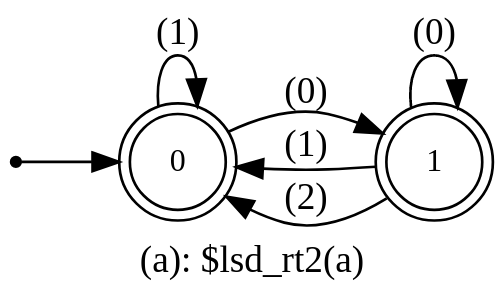
\includegraphics[width=0.4\columnwidth]{lsd_rt2.png}
    \caption{Ostrowski-$\sqrt[~]{2}$ Recognition}
    \label{fig:lsd_rt2}
\end{figure}


%%%%%%%%%%%%%%%%%%%%%%%%%%%%%%%%%%%%%
%% New Section
%%%%%%%%%%%%%%%%%%%%%%%%%%%%%%%%%%%%%
\section{The Addition Algorithm and Corresponding Automaton}


We are interested in creating the following automata which take any $k$-bounded continued fraction $\alpha$ as an input in continued fraction form.

\begin{enumerate}[(i)]
    \item $R_{\alpha}$, which recognizes strings $w$ such that $w$ is a valid Ostrowski-$\alpha$ representation of some natural number $n$.
    \item $<_{\alpha}$, which recognizes pairs $(a,b)_{\alpha}$ such that $a < b$.
    \item $=_{\alpha}$, which recognizes pairs $(a,b)_{\alpha}$ such that $a = b$.
    \item $+_{\alpha}$, which recognizes triples $(a,b,c)_{\alpha}$ such that $a +_{\alpha} b = c$.
\end{enumerate}

In Ostrowski numeration systems, $<_{\alpha}$ is simple to define for any $\alpha$, as we may simply compare the two \word{}s place-by-place.
Similarly, equality of two numbers in an Ostrowski-$\alpha$ numeration system is simply equality on the \letter{}s in the \word{}s.

Recognition can be implemented by following the definition of Ostrowski-$\alpha$ representation, which lends itself to an easy definition in terms of an automaton.
Note that when the expression $1$ is ambiguous, that is, when both $1_{\alpha} = 1$ and $10_{\alpha} = 1$, we choose $10_{\alpha} = 1$ as the unique representation of $1$, as it is the one that matches our definition of a valid Ostrowski-$\alpha$ representation.

Following \citeauthor{ht-ostrowski}, we define four automata which combine to form the bounded addition automaton.

The first of these automata, $\mathcal{A}_0$ takes the Ostrowski-$\alpha$ representations of two natural numbers, $a = x_j x_{j-1} \cdots x_0$ and $b = y_j y_{j-1} \cdots y_0$ and accepts the word $(x_j + y_j) (x_{j-1} + y_{j-1}) \cdots (x_0 + y_0)$.
Note this automaton does not depend on $\alpha$, and therefore does not need to be modified.

The next automaton, $\mathcal{A}_1$ takes this representation and ensures that every symbol is in the proper range, from $0$ to $a_k$, though there may be consecutive symbols which are not allowed in the final representation.
For example, in the Zeckendorf numeration system, that is, the Ostrowski numeration system with $\alpha = \phi$, suppose we add $100_{\phi} + 10_{\phi}$.
The first automaton gives us the new word $110_{\phi}$, and the second automaton leaves this word unchanged, as each value is in bounds---however, this is not a valid Zeckendorf representation as it has two consecutive ones.
The next two automata, $\mathcal{A}_2$ and $\mathcal{A}_3$, correct this issue in two passes: $\mathcal{A}_2$ with one right-to-left pass, and $\mathcal{A}_3$ with one left-to-right pass.

Below, we describe the modifications to the original automata to make each accept the continued fraction of $\alpha$, the irrational number defining the numeration system.
By letting the coefficients of $\alpha$ be between $1$ and $k$, we obtain the addition and recognition automata for $k$-bounded Ostrowski numeration system.
The automaton for the characteristic Sturmian word is essentially the same for any $\alpha$: that is, it only cares about the number of zeroes at the end of the Ostrowski-$\alpha$ representation of $n$ to find the $n$-th digit of $C_{\alpha}$.
Using this, we may define a single automaton for every $\alpha \in \alpha_{<k}$, and we write $C_{\alpha}[n]$ to denote it's $n$-th digit.
This allows us to index into any $k$-bounded Sturmian word, and therefore, to automatically decide theorems about such words.

As noted above, $\mathcal{A}_0$ needs no modifications, so we begin with $\mathcal{A}_1 = (S_1, I_1, T_1, F_1)$.
The set of states, $S_1$, is given by:
\begin{equation*}\label{def:alg1-states}
    S_1 := \Sigma_k^3 \times \Sigma_{2k+1}^3 \times \Sigma_k^3 \times \{0,1\}
\end{equation*}

The initial state, $I_1$ is $((0,0,0),(0,0,0),(0,0,0),0)$.

The transition function is given below, and comes from the rules A1-A3 defined in Algorithm 1~\cite{ht-ostrowski}.
The domain is the subset of the tuples $S_1 \times \{1,\ldots,k\} \times \Sigma_{2k+1} \times \Sigma_k$ that satisfy one of the following rules.
Below, let $s = ((u_1,u_2,u_3),(v_1,v_2,v_3),(w_1,w_2,w_3),g)$ and $v_4 = v_4' + g$.

\begin{itemize}
    \item[(A1)] If $w_1 = v_1$, $v_2 < u_2$, $v_3 > u_3$, and $v_4 = 0$, then 
    
    $$T_1(s,u_4,v_4',w_4) := ((u_2,u_3,u_4),(v_2 + 1, v_3-(u_3+1),u_4-1),(w_2,w_3,w_4),1)$$
    
    \item[(A2)] If $w_1 = v_1$, $v_2 < u_2$, $u_3 \leq v_3 \leq 2u_3$, and $v_4 > 0$, then
    
    $$T_1(s,u_4,v_4',w_4) := ((u_2,u_3,u_4),(v_2+1,v_3-u_3,v_4-1),(w_2,w_3,w_4),0)$$
    
    \item[(A3)] If $v_1 = w_1$ and $v_2 = w_2$, then
    
    $$T_1(s,u_4,v_4',w_4) := ((u_2,u_3,u_4),(v_2,v_3,v_4),(w_2,w_3,w_4),0)$$
\end{itemize}

Similarly, we define the final states to be the states $s \in S_1$ such that $F_1(s) = (w_1,w_2,w_3)$ holds.
$F_1$ is given by the rules B1-B5 defined in Algorithm 1 and is shown below:

\begin{equation*}\label{def:alg1-final-func}
\begin{split}
    F_1&: S_1 \rightarrow \Sigma_k^3\\
    F_1&(s) := 
    \begin{cases}
        F_1((u_2,u_3,u_4),(v_1 - 1, v_2 + u_2 + 1, 0),(w_1,w_2,w_3),0) & \text{if } g = 1\\
        (v_1 + 1,v_2-u_2-1,u_3-1) & \text{if } v_1 < u_1,v_2 > u_2, v_3 = 0\\
        (v_1 + 1, v_2 - u_2, v_3 - 1) & \text{if } v_1 < u_2, v2 \geq u_2, 0 < v_3 \leq u_3\\
        (v_1 + 1, v_2 - u_2 + 1, v_3 - u_3 - 1) & \text{if } v_1 < u_2, v2 \geq u_2, v_3 > u_3\\
        (v_1, v_2 + 1, v_3 - u_3) & \text{if } v_2 < u_2, v_3 \geq u_3\\
        (v_1,v_2,v_3) & \text{otherwise}
    \end{cases}
\end{split}
\end{equation*}

Below we define the automaton $\mathcal{A}_2 = (S_2, I_2, T_2, F_2)$.
Note that $\mathcal{A}_3$ is just $\mathcal{A}_2$, but processing in reverse order.
We may therefore simply reverse the automaton $\mathcal{A}_2$ to obtain $\mathcal{A}_3$ \reed{cite}.

The set of states, $S_2$, is given by $S_2 := (\Sigma_k^2)^3$.
The initial state is $I_2 = ((0,0),(0,0),(0,0))$.
The transition function, $T_2$, is defined below.
Let $s = ((u_2,u_3),(v_2,v_3),(w_2,w_3))$ below.
Again, its domain is the subset of tuples $S_2 \times \{1,\ldots,k\} \times \Sigma_k \times \Sigma_k$ that satisfy one of the following rules:

\begin{itemize}
    \item If $v_1 < u_1$, $v_2 = u_2$, $v_3 > 0$, and $v_3 - 1 = w_3$, then:
    
    $$T_2(s,u_1,v_1,w_1) := ((u_1,u_2),(v_1+1,0),(w_1,w_2))$$
    
    \item If $v_3 = w_3$, then:
    
    $$T_2(s,u_1,v_1,w_1) := ((u_1,u_2),(v_1,v_2),(w_1,w_2))$$
\end{itemize}

Finally, a state $s \in S_2$ is a final state if $v_1 = w_1$ and $v_2 = w_2$ (i.e., $F_2(s) := (v_1,v_2)$).

We can think of each automaton as a predicate on finite sequences of input symbols.
For example, $\mathcal{A}_0(a,b,c)$ holds when $a + b = c$, where $+$ denotes digit-wise addition.
Using this notation, we define the general bounded addition automaton $+_{\alpha}$ which accepts four inputs: $\alpha$, $x$, $y$, and $z$, and accepts when $x +_{\alpha} y = z$.
We can define this automaton in terms of the four automata defined above and standard logical operators and quantifiers, ensuring that there is an automaton that accepts precisely the desired tuples.

Let $A^R$ denote the reversed automaton of $A$; i.e., if $A$ accepts $x$, then $A^R$ accepts $x^R$.

\begin{equation*}
    x +_{\alpha} y = z
\end{equation*}
\begin{equation*}
    \iff
\end{equation*}
\begin{equation*}
    \exists w : \mathcal{A}_0(x,y,w) \text{ and } \exists r : \mathcal{A}_1^R(a,w,r) \text{ and } \exists s : \mathcal{A}_2(a,r,s) \text{ and } \mathcal{A}_3^R(a,s,z)
\end{equation*}

By running the following command in Walnut, we combine our automata for these sub-algorithms 

{
$$\exists y,x,w ~\text{alg}_0(a,b,w) ~\& ~\text{alg}_1(w,x) ~\& ~\text{alg}_2(x,y) ~\& ~\text{alg}_3(y,c)$$}

Using a similar command, we can generate an addition automaton which also accepts some $k$-bounded continued fraction $\alpha$ as an input.
However, the result automaton, even for $k=2$, is far too large to include here; instead, we show the automaton for the Ostrowski-$\sqrt{2}$ system in Figure~\ref{fig:rt2_addition}, which is a specialized version of the more general $k$-bounded Ostrowski addition automata.

\begin{figure}[h]
	\centering
    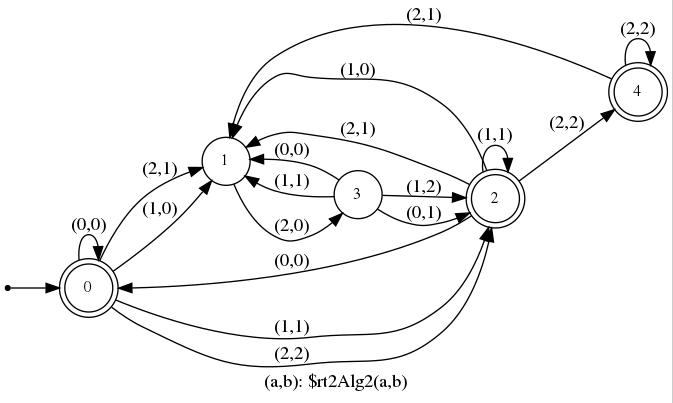
\includegraphics[width=0.6\columnwidth]{rt2Alg2_gv.jpg}
    \caption{Algorithm 2 of Ostrowski-$\sqrt[~]{2}$ (least significant digit first)}
    \label{fig:rt2_alg2}
\end{figure}
\begin{figure}[h]
	\centering
    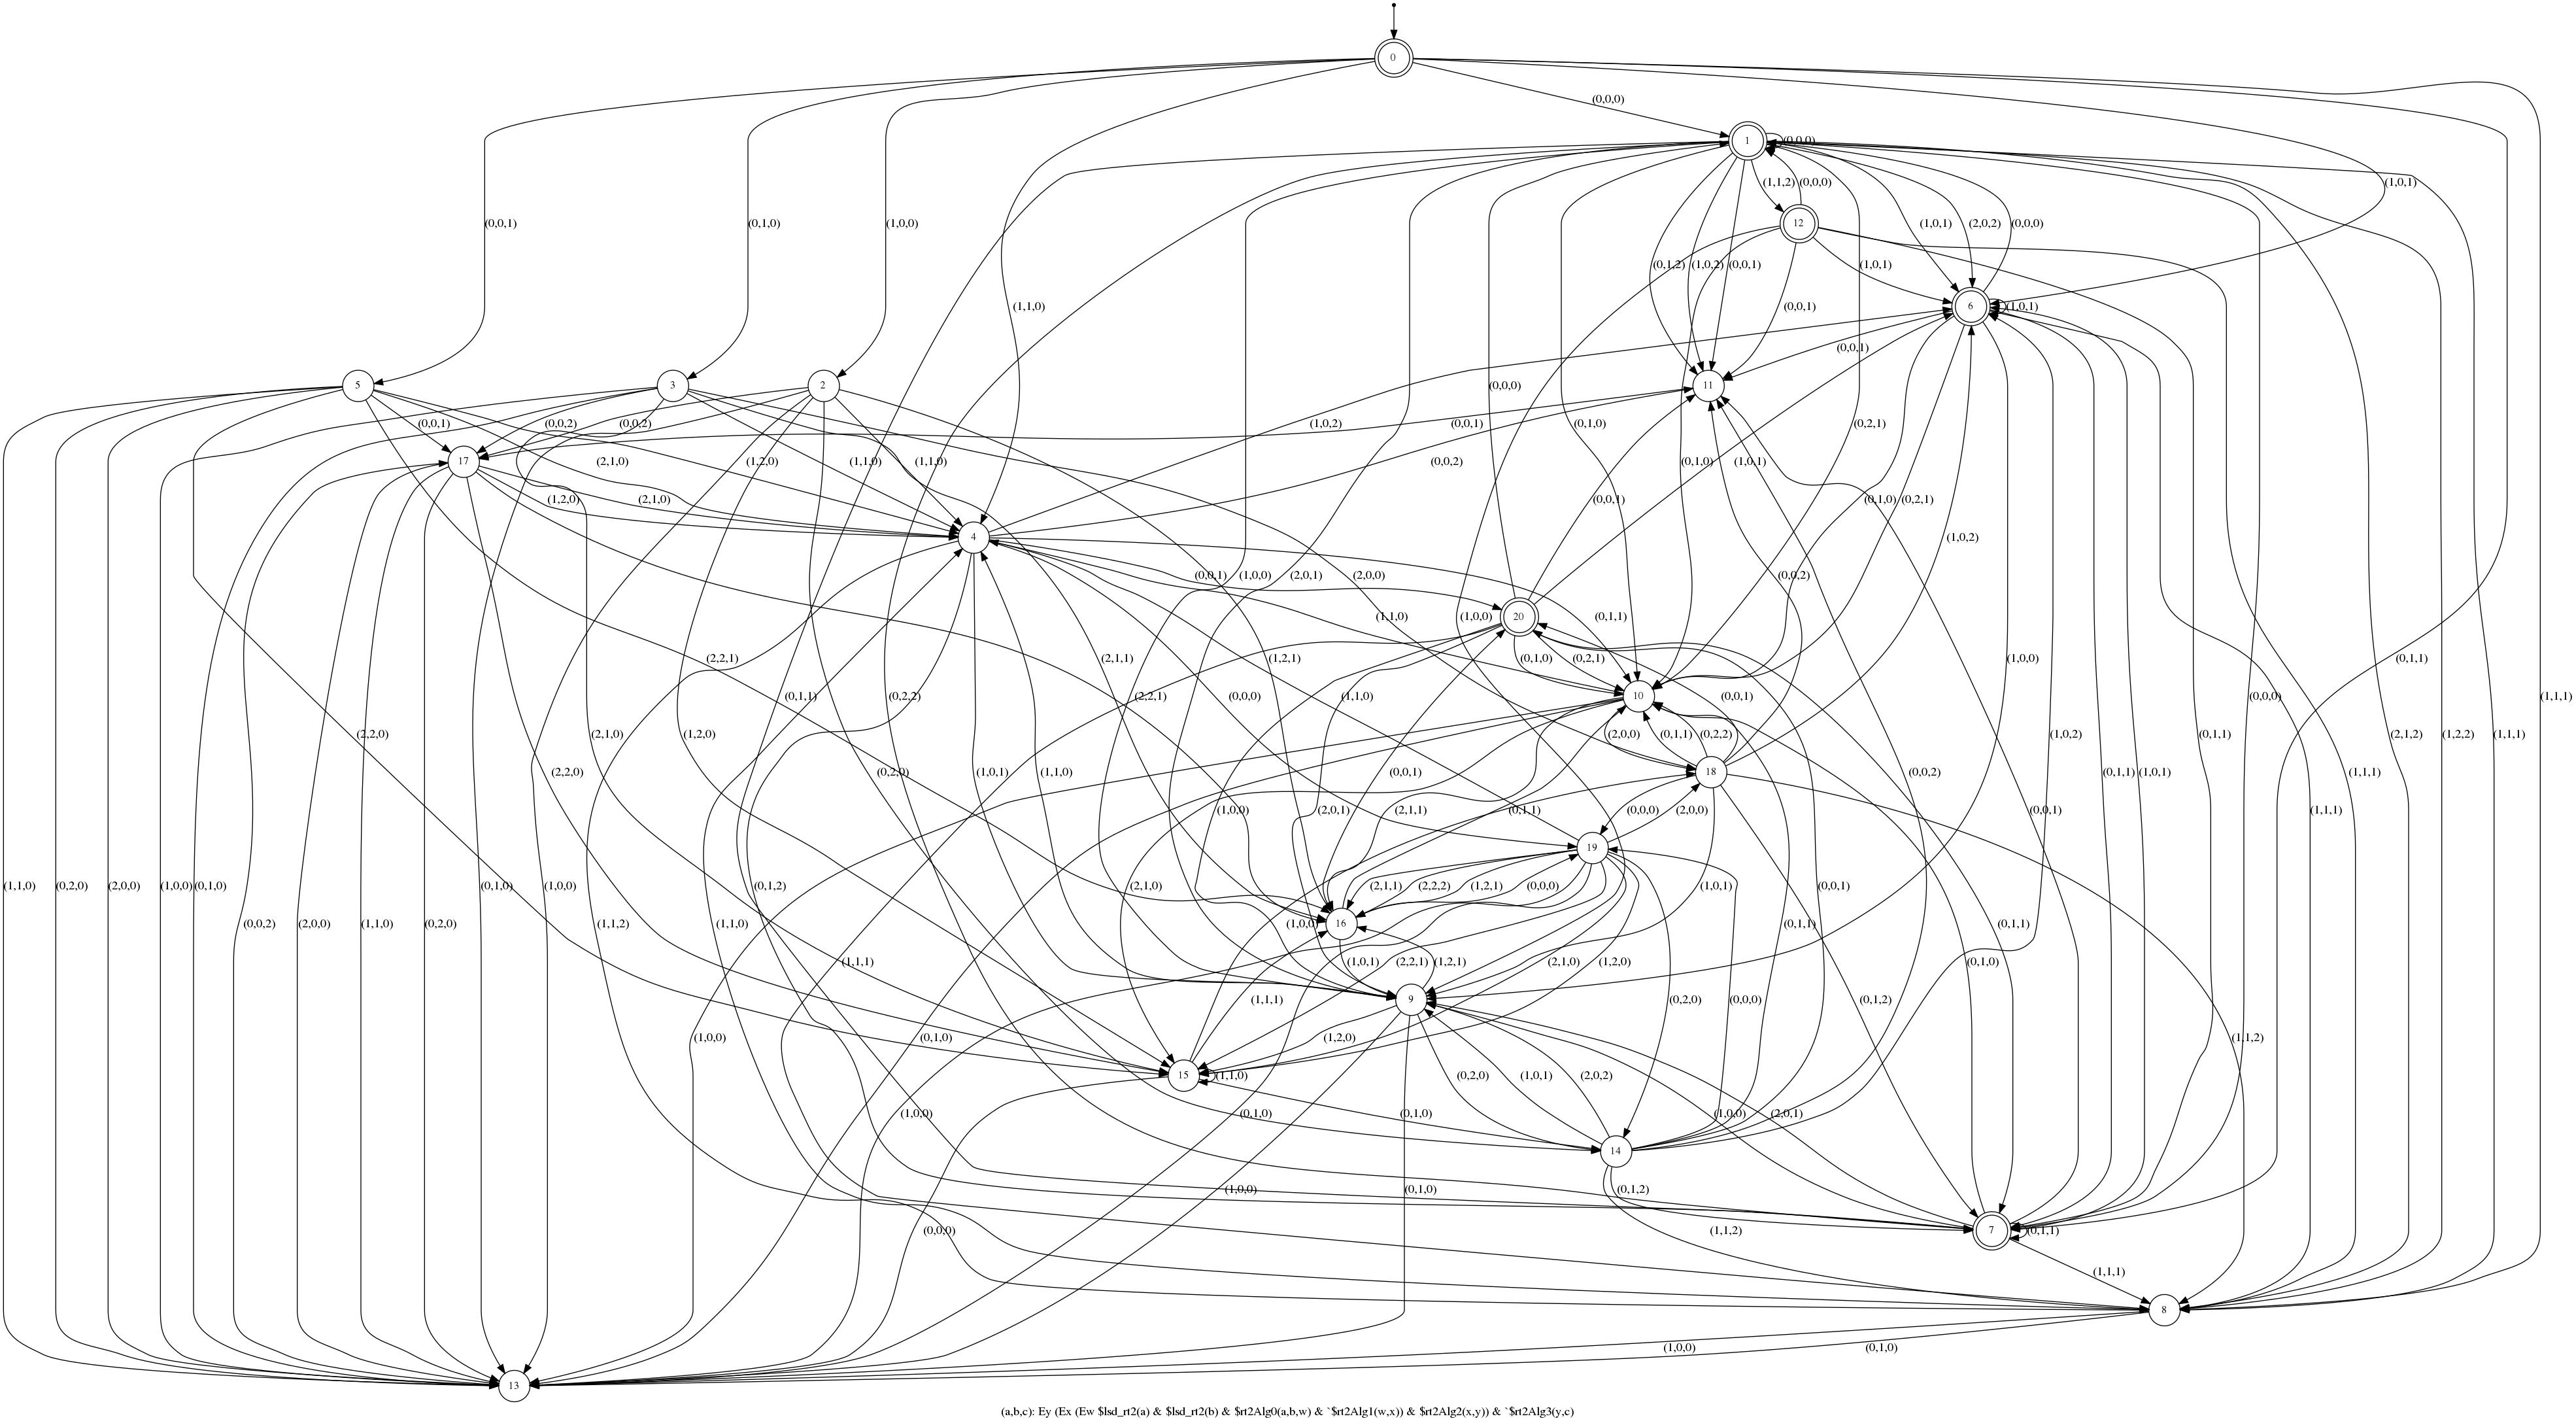
\includegraphics[width=\columnwidth]{lsd_rt2_addition_gv.jpg}
    \caption{Ostrowski-$\sqrt[~]{2}$ Addition}
    \label{fig:rt2_addition}
\end{figure}


%%%%%%%%%%%%%%%%%%%%%%%%%%%%%%%%%%%%%
%% New Section
%%%%%%%%%%%%%%%%%%%%%%%%%%%%%%%%%%%%%

\subsection{Example of addition algorithm in Ostrowski-$\sqrt{2}$}

\begin{minipage}{\columnwidth}
%Insert explanation of Algorithms 1,2 and 3, etc.

We want to add $103_{10}$ and $132_{10}$ in Ostrowski numeration with $\alpha = \sqrt[~]{2}= [1; 2,2,2,\dots].$

\begin{enumerate}
\item Convert into Ostrowski representation:\\
$109_{10} = 0\times1_{10}+0\times2_{10}+2\times5_{10}+0\times12_{10}+1\times29_{10}+1\times70_{10}= 0110200_{\sqrt[]{2}}$
\\
$138_{10} = 0\times1_{10}+0\times2_{10}+2\times5_{10}+0\times12_{10}+2\times29_{10}+1\times70_{10} = 0120200_{\sqrt[]{2}}$
\item Run Algorithm 0 (add operands): $0110200 + 0120200 \Rightarrow 0230400$.
\item Run Algorithm 1 (check constraint 1): $0230400 \Rightarrow 1020400 \Rightarrow 1021111$.
\item Run Algorithms 2 and 3 (check constraint 2): $1021111 \Rightarrow 1100111$. (Try this on \emph{Figure 2}.)
\end{enumerate}

Therefore, $0110200_{\sqrt[]{2}}+0120200_{\sqrt[]{2}}=1100111_{\sqrt[]{2}}$.

Verify:
$1100111_{\sqrt[]{2}}  = 1\times1_{10}+1\times2_{10}+1\times5_{10}+1\times70_{10}+1\times169_{10}$ = $247_{10} = 109_{10}+138_{10}$.\\

\end{minipage}

%%%%%%%%%%%%%%%%%%%%%%%%%%%%%%%%%%%%%
%% New Section
%%%%%%%%%%%%%%%%%%%%%%%%%%%%%%%%%%%%%
\section{Characteristic Sturmian word}

%include theorems, yay!
With the definition of the automaton for addition in Ostrowski numeration systems, we were able to construct similar proofs as those in Du, Mousavi, Schaeffer, and Shallit's study \cite{fibonacci} for the \textbf{characteristic Sturmian word with slopes $\sqrt[~]{2}$ and $\sqrt{3}$} rather than the original Fibonacci word.
We also used the new automaton for $k$-bounded Sturmian words to produce results for 

% \vspace{0.4em}
\begin{definition}
The \textbf{characteristic Sturmian word with slope $\alpha$}, which we denote as $C_{\alpha}$, is the infinite word obtained as the limit of the sequence of \textbf{standard words} $s_n$ defined by{

$$ s_n=s^{d_n}_{n-1}s_{n-2} \text{ when } n\ge 2, \text{ where } s_1= 0^{d_1-1}1 \text{ and } s_0=0.$$}

where the $d_n$ are the coefficients of the continued fraction representation of $\alpha$.
\end{definition}

By having built the Ostrowski-$\alpha$ numeration system and the automatic word $C_{\alpha}$ in Walnut, we may use the command $C_{\alpha}[i]$ to return the $i^{th}$ digit of $C_{\alpha}$ with the following theorem:\\

\begin{theorem}[\cite{auto_seq}, Theorem 9.1.15] Let $N \geq 1$ be an integer with Ostrowski$\alpha$-representation $b_jb_{j−1}\cdots b_0$. Then $C_\alpha[N] = 1$ if and only if $b_jb_{j−1}\cdots b_0$ ends with an odd number of $0$’s.
\end{theorem}


In this section, we include the theorems proven using our automata for both regular and bounded Ostrowski addition and Sturmian words.
Proofs have been omitted for brevity.

\section{Mechanical proofs of properties of Sturmian words}\label{sec:specific-theorems}

In this section we expand on the study done in \reed{Fibonacci word paper} with several new values for $\alpha$: $\sqrt{2}$ and $\sqrt{3}$.
We use these theorems to show the capabilities of our approach and to provide inspiration into what sorts of generalizations we may investigate using our new automata for $k$-bounded Sturmian words.

The words $\Ctwo$ and $\Cthree$ start as shown below:

\begin{itemize}
    \item[$\Ctwo$:] $01010010100101 \ldots$
    \item[$\Cthree$:] $11011101110110 \ldots$
\end{itemize}

%%%%%%% Section 3.1 %%%%%%%
\subsection{Aperiodicity}
%%%%%%% Theorem 4 %%%%%%%

We start with the well-known theorem that Sturmian words are not ultimately periodic.

\begin{theorem}\label{thm:ulti_period_C}
The \word{}s $\Ctwo$ and $\Cthree$ are not ultimately periodic.
\end{theorem}

\subsection{Palindromes and antipalindromes}

\begin{definition}
A string $s$ is a \emph{palindrome} if its reverse is the same as itself, that is, when $s = s^R$.
\end{definition}

\begin{definition}
A string $s$ is \emph{mirror invariant} if for any factor $x$, the reverse $x^R$ is also a factor of $s$.
\end{definition}

\begin{definition}
A string $s$ is an \emph{antipalindrome} if its reverse is the complement of itself, that is, when $s = \overline{s^R}$.
\end{definition}

\begin{theorem}
$\Ctwo$~ and $\Cthree$ contains antipalindromes of all lengths.
\end{theorem}

%%%%%%%%%%%%%%%%%%%%%% Theorem 13 %%%%%%%%%%%%%%%%%%%%%%
\begin{theorem}
$\Cthree$ ~contains exactly one palindrome of length $n$ if and only if $n$ is odd. 
\end{theorem}

\begin{theorem}
$\Ctwo$ and $\Cthree$ are mirror invariant. 
\end{theorem}

\begin{theorem}
The only nonempty antipalindromes in $\Ctwo$ are 01, 1001, and 010010.\\
The only nonempty antipalindromes in $\Cthree$ are 01 and 10.
\end{theorem}

\subsection{Special factors}
Next we will prove that \Ctwo and \Cthree \ have exactly n + 1 distinct factors of length n, for each n $\geq$ 0.  This implies that there is exactly one factor x of each length n with the property that both x0 and x1 are factors. Such a factor is called right-special or just special.  

\begin{theorem}
The unique special factor of length n is $C[0\ldots n-1]^{R}$, where C = \Ctwo\ or \Cthree
\end{theorem}

\subsection{Quasiperiods}

An infinite word \textbf{a} is said to be \term{quasiperiodic} if there is some finite nonempty word $x$ such that $a$ can be completely ``covered" with translates of $x$. 
We study the stronger version of quasiperiodicity where the first copy of $x$ used mys be aligned with the left edge of \textbf{w} and is not allowed to ``hang over"; these are called \term{aligned covers}. 
For us $\mathbf{a} = a_{0}a_{1}a_{2}...$ is quasiperiodic if there exists $x$ such that for all $i>0$ and $i>n$ there exists $j>0$ with $i-n<j\leq i$ such that $a_{j}a_{j+1}...a_{j+n-1}=x$, where $n=|x|$. Such an $x$ is called a \term{quasiperiod}. 

\begin{theorem}
A nonempty length-$n$ prefix of $\Ctwo$ is a quasiperiod of $\Ctwo$ if and only if $n$ is not in the form $P_n - 1$ or $P_n + P_{n-1} - 1$, where $P_n$ are Pell numbers.
\end{theorem}

\subsection{Recurrence, uniform recurrence, and linear recurrence}

A \factor $x$ of infinite \word $C$ is said to be \term{recurrent} if it occurs infinitely many times in $C$. 
An infinite \word $C$ is \term{recurrent} if every factor of $C$ is recurrent. 
A \factor $x$ is \term{uniformly recurrent} if there exists a length $n = n(x)$ such that every factor of length $n$ contains $x$.
An infinite word is uniformly recurrent if all factors of its factors are uniformly recurrent.
If $n(x)$ is in $O(x)$ for all factors $x$, then $C$ is linearly recurrent. 

Notice that linear recurrence implies uniform recurrence and recurrence.

\begin{theorem}
$\Ctwo$ and $\Cthree$ are linearly recurrent. 
\end{theorem}

\subsection{Lyndon words}

A nonempty word $x$ is a \textit{Lyndon word} if it is lexicographically less than all of its nonempty proper prefixes. For example, in $C_{\sqrt{2}}$, 120 is a Lyndon word as it is lexicographically less than its rotations, 201 and 012, in lsd.

\begin{theorem}
In $C_{\sqrt{2}}$ and $C_{\sqrt{3}}$, there exists a Lyndon factor of all lengths n.
\end{theorem}

\begin{theorem}
For $n \geq 1$, every length-$n$ Lyndon factor of $C_{\sqrt{2}}$ or $C_{\sqrt{3}}$ is a conjugate of $C_{\sqrt{2}}(1, n)$ or $C_{\sqrt{3}}(1, n)$ respectively.
\end{theorem}

\subsection{Critical Exponents}
Define exp(\textit{w}) as $|\textit{w}|$/\textit{P}, where \textit{P} is the smallest period of \textit{w}. 
The \textit{critical exponent} of an infinite word \textbf{x}, is the supremum, over all factors $w$ of \textbf{x}, of exp(\textit{w}).

\begin{theorem}
The critical exponent of $C_{\sqrt{2}}$ is $4 + 2\sqrt{2}$.
\end{theorem}

\subsection{The Shift Orbit Closure}

The \term{shift orbit closure} of a \word $x$ is the set of all \word{}s $t$ with the property that each prefix of $t$ appears as a \factor of $x$.

\begin{theorem}
The lexicographically least sequence in the shift orbit closure of C is 0C, and the lexicographically greatest is 1C where C = \Ctwo\ or \Cthree. 
\end{theorem}

\subsection{Aperiodicity}

\begin{conjecture}
For all $k \ge 1$, $k$-bounded Sturmian words are not ultimately periodic.
\end{conjecture}

We are able to check for the case up for $k=5$.

\subsection{Squares in bounded Sturmian words}

A factor $z$ is called a \term{square} if can be written as $z = xx$ for some word $x$.
The \term{order} of a square is the length of the repeated part, $|x|$.

\begin{conjecture}\label{conj:square}
    When $k > 2$, the orders of the squares in $k$-bounded Sturmian words are of the form $E_k = (1+2+\cdots+(k-1))(1+\epsilon)0^*$.
    That is, they are either a single digit, from $1$ to $k-1$ followed by arbitrarily many zeroes; or a single digit from $1$ to $k-1$, followed by a $1$, followed by arbitrarily many zeroes.
\end{conjecture}

\begin{theorem}\label{thm:square-conj-prf}
Conjecture~\ref{conj:square} holds for $k \in \{1,2,3,4,5\}$.
\end{theorem}

\subsection{Antisquares in bounded Sturmian words}

A factor $z$ is called an antisquare when it is of the form $z = x\overline{x}$ for some word $x$.

We conjecture the following:

\begin{conjecture}\label{conj:antisq}
    For every characteristic Sturmian word with slope $\alpha$, there are finitely many antisquare factors in $C_{\alpha}$.
    Furthermore, every antisquare is either a palindrome or an antipalindrome.
\end{conjecture}

\begin{theorem}\label{thm:antisq}
Conjecture~\ref{conj:antisq} holds for all $\alpha \in \alpha_{\leq k}$ when $k \in \{1,2,3,4,5\}$.
\end{theorem}

\subsection{Approximate antisquares}

Let $C_{\alpha}$ be a Sturmian word, and $x$ a \factor in $C_{\alpha}$ such that $x=uv$ where $|u| = |v|$.
Consider the Hamming distance, $H(u,v)$, which is the number of places in which $u$ and $v$ differ.
Define $S(u,v)$ to be the number of places for which $u$ and $v$ are the same when $|u| = |v|$.
Note that $S(u,v) + H(u,v) = |u|$, if $S(u,v) = |u|$, then $uv$ is a square, and if $S(u,v) = 0$, then $uv$ is an antisquare.

We call a \word $x$ an \term{$\ell$-approximate antisquare} if $x = uv$ such that $|u| = |v|$ and $S(u,v) \leq \ell$, that is, where $u$ and $v$ have at most $\ell$ characters in the same place.
Note $0$-approximate antisquares are precisely the antisquares in the usual sense.
We conjecture the following:

\begin{conjecture}\label{conj:approx-antisq}
    The set of $\ell$-approximate antisquares in $C_{\alpha}$ is finite for every $\ell$ and $\alpha$.
\end{conjecture}

\begin{theorem}\label{thm:approx-antisq}
Conjecture~\ref{conj:approx-antisq} holds when $k = 2$ and $\ell = 1$, and when $k \leq 5$ and $\ell = 0$.
\end{theorem}

\subsection{Higher-Order Powers}

\begin{conjecture}
    For all $k\ge 1$, $k$-bounded Sturmian words does not contain a $(k+3)^{th}$ power.
\end{conjecture}

\begin{conjecture}
    Let $\alpha$ be a quadratic irrational number, if the maximum of the repeated part of the continued fraction of $\alpha$ is $k$, then the Sturmian word with slope $\alpha$ contains a $(k+2)^{th}$ power.
\end{conjecture}

\subsection{Unbordered factors in Sturmian words}\label{sec:unbordered}

A \word $w$ is said to be \term{bordered} if there is some \word $u$ and some nonempty \word $x$ such that $w = xux$.
A \word $w$ is unbordered if there is are no such \word{}s $u$ and $x$.

\citeauthor{fibword} found that all unbordered \factor{}s of the Fibonacci word have length $F_n$ for some Fibonacci number $F_n$ with $n \geq 2$.
Furthermore, there are exactly two \factor{}s for each length $F_n$, and one is the reverse of the other.

\begin{conjecture}\label{conj:unbordered}
    If $x$ is an unbordered \factor in some $k$-bounded Sturmian word $w$, then $|x|$ is of the form $N0^*$ where $N$ is some \word in $\{1,\ldots,k\}^+$.
\end{conjecture}

\begin{theorem}\label{thm:unbordered}
Conjecture~\ref{conj:unbordered} holds for $k = 5$.
\end{theorem}

\subsection{Grouped factors}

We say an infinite \word $w$ contains \term{grouped factors} if, for all lengths $n > 0$, there exists a \factor $z$ that contains all the  length $n$ \factor{}s of $w$.
Furthermore, each length-$n$ \factor of $w$ occurs exactly once in $z$.
We call this \factor $z$ the \term{grouped factor for length $n$}.
The following predicate is true if and only if $C$ contains grouped factors.
The first part states the existence of each length-$n$ \factor in $w = C[m \ldots s]$, and the second states the uniqueness.

\begin{conjecture}\label{conj:grouped}
    Every Sturmian word contains grouped factors.
\end{conjecture}

We are able to verify Conjecture~\ref{conj:grouped} for $k=3$.


\section{Future Work}
\begin{itemize}
\item Use the automata for Ostrowski numeration systems to prove more theorems regarding characteristic Sturmian words.
% \item Investigate the critical exponent of infinite balanced words.
\item Find a faster algorithm to generate automata for bounded Ostrowski addition.
\item Provide a general automaton for Ostrowski numeration, which would accept any $\alpha$ as an input, with no bound on the coefficients.
\end{itemize}

\printbibliography

\end{document}
